This section present an analysis of the microstructure based on the nearest pair probability density function.%age included nearest pair probability density function  $P_\text{nst}(\textbf{x},\textbf{r},t,a)$ and on .
After identifying the different forms of the microstructure with respect to the dimensionless parameters, we introduce a general and concise way to quantify it.


\subsubsection*{Low inertial effects }
We begin with a detailed analysis of $P_\text{r}^n$ at $Ga =10$, to investigate the influence of $\lambda$ and $\phi$ on the microstructure when inertia effects are low.
As it will be seen in the next section the nearest particle statistics does not show fore-aft symmetry with respect to the horizontal plane, as it is the case for classic particle pair statistics. 
Nevertheless, it turns out that $P_\text{r}$ possesses a nearly symmetric distribution, such that $P_\text{r}^n(\textbf{x},t,r,\theta)\approx P_\text{r}^n(\textbf{x},t,r,- \theta)$. 
Therefore, in the following plots, displayed in \ref{fig:Pnst_low_Ga} and \ref{fig:Pnst_high_Ga}, we choose to show only the upper part of the distribution.
Additionally, in the discussion below we refer to the sphere at the origin of the graphs, located at $\textbf{x}=0$, as the \textit{reference particle}.%\textit{test particle} or the \textit{reference particle}. 

\begin{figure}[h!]
    \centering
    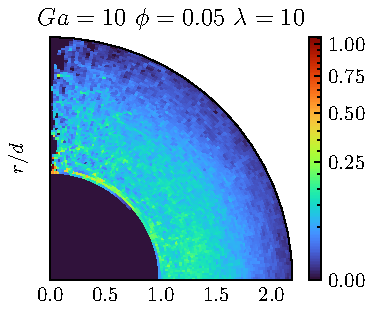
\includegraphics[height=0.21\textwidth]{image/HOMOGENEOUS_NEW/Dist/Pnst_l_10_Ga_10_PHI_0_05.pdf}
    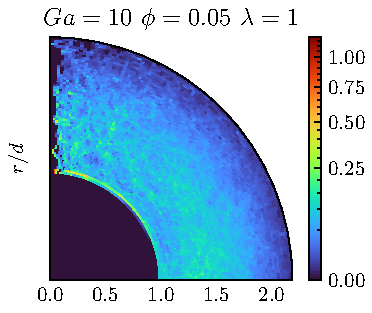
\includegraphics[height=0.21\textwidth]{image/HOMOGENEOUS_NEW/Dist/Pnst_l_1_Ga_10_PHI_0_05.pdf}
    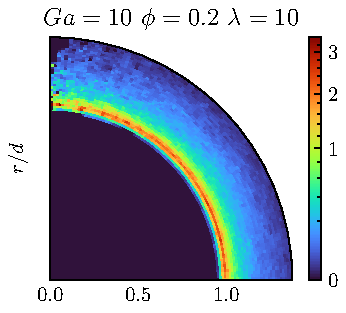
\includegraphics[height=0.21\textwidth]{image/HOMOGENEOUS_NEW/Dist/Pnst_l_10_Ga_10_PHI_0_2.pdf}
    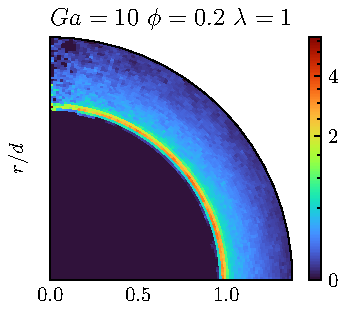
\includegraphics[height=0.21\textwidth]{image/HOMOGENEOUS_NEW/Dist/Pnst_l_1_Ga_10_PHI_0_2.pdf}
    \caption{Histogram of the normalized function, $P_\text{r}^n$, at low inertial effects $Ga = 10$.
    The color map represents the nearest pair distribution function. %the values of $P_\text{r}^n$.
    The origin corresponds to the position of the reference particle.
    The dimensionless radial and azimuthal coordinates, $|\textbf{r}|/d$ and $\theta$, correspond to the nearest neighbor position.
    The vertical direction corresponds to the flow direction, which is also the axis of symmetry for $P_\text{r}^n$.
    (left) Low volume fraction cases $\phi=0.05$ for $\lambda = 1,10$.
    (right) High volume fraction cases $\phi=0.2$ for $\lambda = 1,10$.}
    \label{fig:Pnst_low_Ga}
\end{figure}
The first observation from \ref{fig:Pnst_low_Ga} indicates that the likelihood of finding the nearest neighboring particle at an angle $\theta$ is uniform across all $\theta$.
This suggests that $P_\text{r}^n$ is isotropic at these \textit{Galileo} numbers. We can observe that $P_\text{r}^n$ is larger close to the reference particle ($r/d = 1$) in the high volume fraction cases than in the low volume fraction cases.
%If we compare the low volume fraction cases to the high volume fraction cases, we can observe that $P_\text{r}^n$ is larger at near contact of the test particle ($r/d = 1$) in the latter case.
For solid particles it is also common that pair distributions are more concentrated at the contact of the test particle for increasing $\phi$. 
In practice, if particles are more likely to be close to one another, it means that densely packed regions of particles are present in the flow.
This suggests that isotropic clusters, as represented in \ref{fig:scheme_clusters} (\textit{Case 2}), are likely to form in the present context.% emulsion or suspension. 
Regarding the effect of the viscosity ratio, $P_\text{r}^n$ are very similar for both values of $\lambda$ except that for the highest volume fraction the region of highest probability is thinner for the lowest aspect ratio. 
Consequently, in this regime we find homogeneous microstructures at low $\phi$, and non-homogeneous but still isotropic microstructure at higher $\phi$. 

